\documentclass[pdftex,12pt,a4paper]{article}

\usepackage{graphicx}  
\usepackage[margin=2.5cm]{geometry}
\usepackage{breakcites}
\usepackage{indentfirst}
\usepackage{pgfgantt}
\usepackage{pdflscape}
\usepackage{float}
\usepackage{epsfig}
\usepackage{epstopdf}
\usepackage[cmex10]{amsmath}
\usepackage{stfloats}
\usepackage{multirow}

\renewcommand{\refname}{REFERENCES}
\linespread{1.3}

\usepackage{mathtools}
%\newcommand{\HRule}{\rule{\linewidth}{0.5mm}}
\thispagestyle{empty}
\begin{document}
\begin{titlepage}
\begin{center}
\textbf{}\\
\textbf{\Large{ISTANBUL TECHNICAL UNIVERSITY}}\\
\vspace{0.5cm}
\textbf{\Large{COMPUTER ENGINEERING DEPARTMENT}}\\
\vspace{2cm}
\textbf{\Large{BLG 222E\\ Computer Organization \\ Project 2}}\\
\vspace{2.8cm}
\begin{table}[ht]
\centering
\Large{
\begin{tabular}{lcl}
\textbf{PROJECT DATE}  & : & 24.05.2023\\
\end{tabular}}
\end{table}
\vspace{1cm}
\textbf{\Large{GROUP MEMBERS:}}\\
\begin{table}[ht]
\centering
\Large{
\begin{tabular}{rcl}
150220762  & : & Muhammed Yusuf Mermer (Group Representative)  \\
150210071  & : & Emre Çamlıca \\
150200091  & : & Hakan Duran \\
\end{tabular}}
\end{table}
\vspace{2.8cm}
\textbf{\Large{SPRING 2023}}

\end{center}

\end{titlepage}

\thispagestyle{empty}
\addtocontents{toc}{\contentsline {section}{\numberline {}FRONT COVER}{}}
\addtocontents{toc}{\contentsline {section}{\numberline {}CONTENTS}{}}
\setcounter{tocdepth}{4}
\tableofcontents
\clearpage

\setcounter{page}{1}
\section{INTRODUCTION}
In this project our purpose was to design a hardwired control unit. To achive this we divided it into parts. Yusuf did 
the fetch and decode parts, Hakan did the instructions without memory reference and Emre did the instructions with 
memory reference parts. Yusuf also wrote the test bench and tested the system with Hakan. 

We used the ALU System module to determine the paths we should go through in order to implement the operations 
determined by the instruction register. Then we designed the operations, using the selectors and multiplexers to choose
the right values. After that, we tested the general project and made corrections in order to make it work properly, 
according to the example memory cycle given. 

\section{IMPLEMENTATIONS AND EXPLANATIONS }
\subsection{Fetch Cycle, Counter and Decoding}
In our implementations, we made only counter module seperated from the 
combined system. It could have also been designed inside of overall 
combined system as a register, but this was our design choice. It takes 
clock as input, because at every positive edge we increase our timing signal
by 1. However, to prevent unexpected result in the current postive edge we wait for
0.25 ns in our implementation.

Not only clock, but also reset signal taken as input for this module
to return inital value for the timing signal. When it reset, it returns value 4 bit
binary 1111 which is equal to -0001, this is been made because reset signal 
does not depend on clock; therofore, after the reset we wait for new clock signal 
to start new operations. New operations will be started with timing signal 0.

Inside of inital block, we make all register values 0 for use in the operations.
Then to prevent further changes we closed rsel and tsel values.

We have 3 always block inside of our implementations. Our very first always
 block works at every new instruction. It closes all rsels and tsels and also
 closes IR enable. Also after reseting signal, we need to make reset command
 0 to prevent always 0 problem of counter.

2nd always block, works similar to 1st one but it doesn't reset at every time,
because this operation doesn't needed. In here our purpose is to close all
registers from changing their values with the incoming new timing signal.


After making all necesessary connections, in 3rd always block, when timing signal 0 
arrives to our combined system, it starts to fetch cycle. Our 
fetch cycle is totally takes 3 cycles. It has been made 3 cycles to prvent 
changes unintended changes on the PC and IR.



At first (0th) cycle of the fetch, we just pushed values of M[PC] to the IR's LS 8 bits.
This because memory can only give 8 bit output at once. To do this operation, we give PC
as adress to memory.

At second (1st) cycle, we only increased PC value by one. To do this, we just opened PC's
register for input changes and send increment by one signal to funsel of arf.

At last (2nd) cycle, we do combined operations of 0th and 1st cyles, but different than 0th,
this time high bits of IR will be changed.



For decoding part (3th cycle), for the opcodes that addresing mode doesn't requried, we made a simple output opener.
In other words, our module looks at here to decide where to take sreg's. It depends on the where register resits. If [2] bit
is 0 it means that it will be RF, if 1 it will be ARF. The pattern of RF same for [1:0], so we did not
make a change end send them directly. However for ARF, we used switch case for manipulation.


At the end of every insturction, we need to send a reset signal, so depending 
on the opcode type, we will send request for reset. When all operations are finished 
for a instuction, this operations occurs in the next clock cycle.






\subsection{Instructions With Address Reference}
Instructions that have address references either write something on memory or execute a task coming from the chosen 
memory address. 

\subsubsection{BRA}
In this operation, the adrress block of the instruction register is directly written into the program counter.

To do this, the MUX B is selected as "10" to choose the input coming from the IR. The Regsel 
input of the ARF is chosen as "0001" which activates only the PC and the Funsel input of the ARF is "01" indicating
the load mode.

\subsubsection{BNE}
This operation is exactly the same as the "BRA" operation except that it checks zero flag of the ALU. If it is zero,
the condition is met and the operation is done.

\subsubsection{LD}
This operation is implemented differently, depending on the addressing mode of the instruction.

If the addressing mode is immediate addressing, indicated by "0", the address in the IR is written into a register
chosen by the register selection bits of the instruction. To do this, MUX A is selected as "10" to choose the input 
coming from the IR. The Funsel of RF is chosen as "01", indicating the load mode. The register to load is selected 
using a case statement, depending on the value of the register selection bit of the instruction.


If the addressing mode is direct addressing firstly, the value of the address register is given as address to the 
memory which is indicated by the outDsel of the ARF being "00". Then, MUX A is selected as "01" to choose the input 
coming from the memory. The Funsel of RF is chosen as "01", indicating the load mode. The register to load is selected 
using a case statement, depending on the value of the register selection bit of the instruction.

\subsubsection{ST}
In this operation, the value in a register selected by the register selection bits of the IR is written to the memory
location determined by the address register. 

First, the D output of the ARF is selected as "00", so that the AR is given as address to memory. The register that 
will write to the memory is again chosen by the register selection bits of the instruction, using a case statement.
Then, the MUX C is selected as "0" to give the chosen register as the input to ALU. The ALU directly transfers the 
value in the selected register to the memory, as the funsel is "0000". Then, the value is written into the desired
memory location.

\subsubsection{PUL}
In this operation, the value in the memory address determined by the stack pointer is written into a register. 
Then, the value of the SP is incremented.

First, the D output of ARF is selected as "01" to give the SP as an address to the memory. Then, MUX A is selected
as "01" in order for it to take the input coming from the memory. The Funsel of RF is chosen as "01", indicating the
load mode. The register to load is selected using a case statement, depending on the value of the register selection
bit of the instruction. In the next cycle, the value of SP is incremented using the ARF registers increment operation.

\subsubsection{PSH}
In this operation, the value in a register is written into the memory location determined by the stack pointer.
Then, the value of the SP is decremented.

First, the D output of ARF is selected as "01" to give the SP as an address to the memory. Then, the register is 
selected depending on the value of the register selection bit of the instruction, that will be given as input to ALU.
The MUX C is selected as "0" to take the input from the RF. The ALU directly conveys the value in the register with 
the "0000" coded operation, so that the value in the register is written into the memory. In the next cycle, the value 
of SP is incremented using the ARF registers increment operation.


\subsection{Instructions Without Address Reference}
    Instructions without address references have four seperate fields whose functionalities differ. Each one has 4 bits. Opcode determines which operation
will be carrying out. DSTREG means destination register, SREG1 and SREG2 are source registers. There are 10 instruction types.
\subsubsection{AND}
    AND operation's opcode is 0x00. It carries out by determining ALU Funsel as 0111.
\subsubsection{OR}
    OR operation's opcode is 0x01. It carries out by determining ALU Funsel as 1000.
\subsubsection{NOT}
    NOT operation's opcode is 0x02. It carries out by determining ALU Funsel as 0010.
\subsubsection{ADD}
    ADD operation's opcode is 0x03. It carries out by determining ALU Funsel as 0100.
\subsubsection{SUB}
    SUB operation's opcode is 0x04, it is responsible for substract operations. It carries out by determining ALU Funsel as 0101.
\subsubsection{LSR}
    LSR operation's opcode is 0x05, it is responsible for logical shift right operations. It carries out by determining ALU Funsel as 1100.
\subsubsection{LSL}
    LSL operation's opcode is 0x06, it is responsible for logical shift left operations. It carries out by determining ALU Funsel as 1011.
\subsubsection{INC}
    INC operation's opcode is 0x07, it is responsible for increment operations. It carries out by determining ALU Funsel as 0100.
It takes 3 cycles because in order to increment and then send to ALU, we should first create a register
which has value 1. Making it takes 2 cycle, first cycle for using a temporary register which has value 0.
Then in second cycle, we make it 0001 with incrementing and use it in ALU.
\subsubsection{DEC}
    DEC operation's opcode is 0x08, it is responsible for decrement operations. It carries out by determining ALU Funsel as 0101.
It takes 3 cycles because in order to decrement and then send to ALU, we should first create a register
which has value 1. Making it takes 2 cycle, first cycle for using a temporary register which has value 0.
Then in second cycle, we make it 0001 with incrementing and use it in ALU.
\subsubsection{MOV}
    MOV operation's opcode is 0x0B. It carries out by determining ALU Funsel as 0000.


\section{OVERALL DESIGN PHOTO}


\begin{figure}[H]
    \centering
    \includegraphics[width=1\textwidth]{photos/design.png}	
    \caption{overall design photo}
    \label{implementation}
\end{figure}








\section{SIMULATION RESULTS}


\begin{figure}[H]
    \centering
    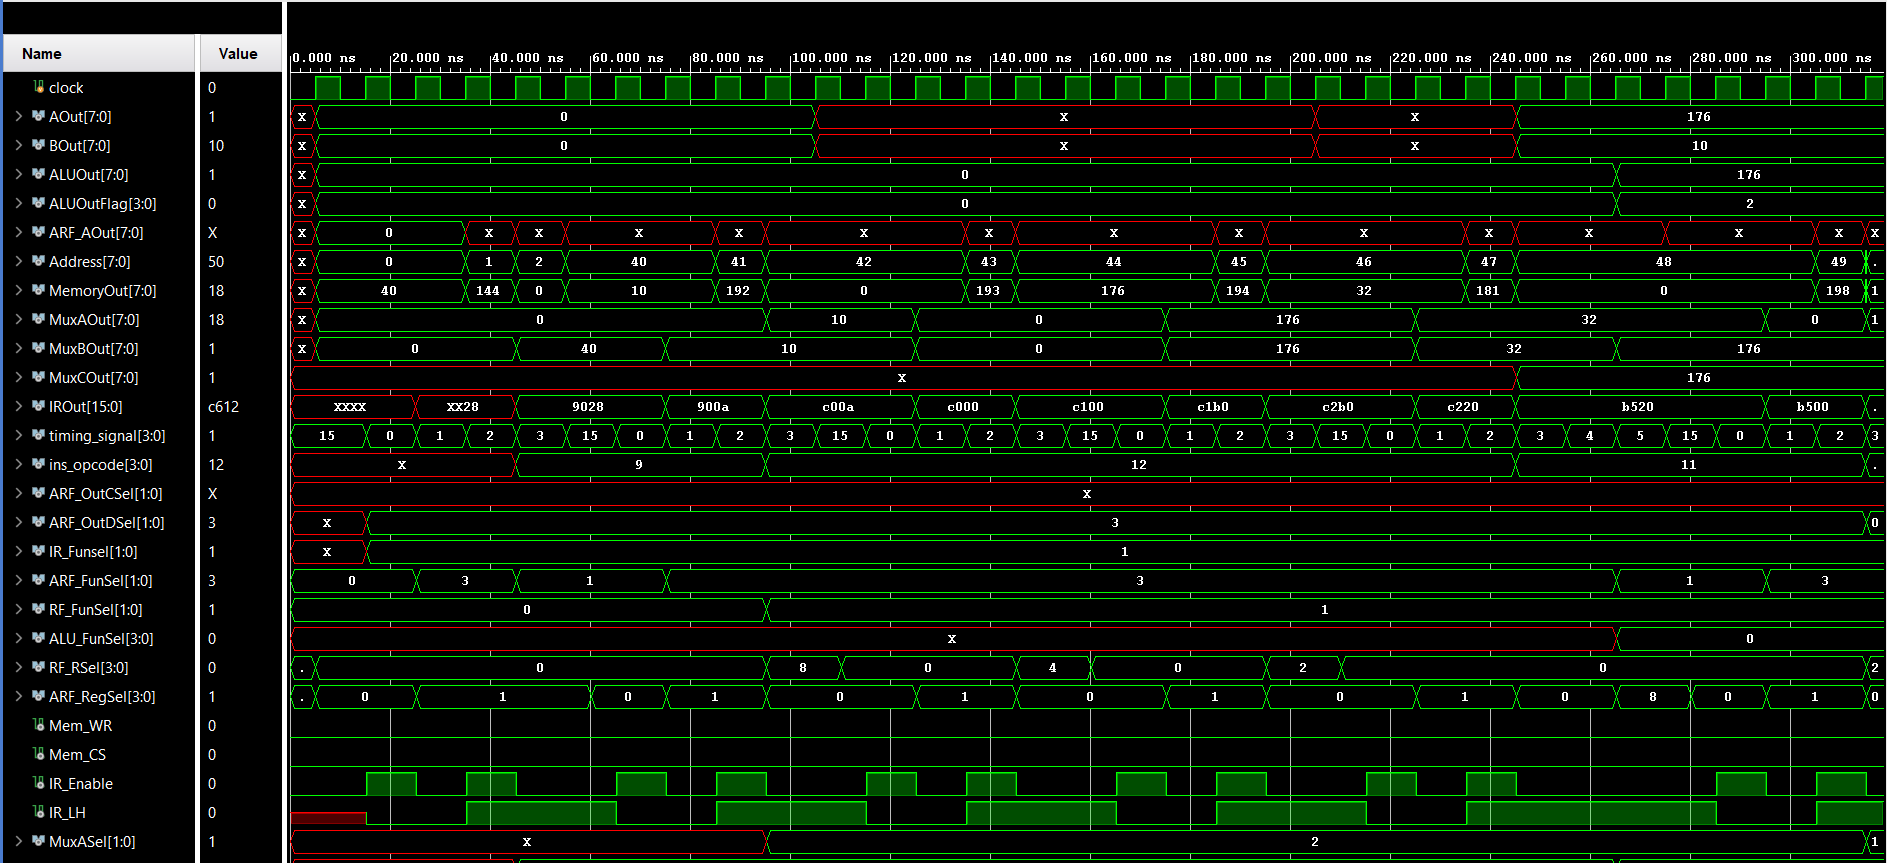
\includegraphics[width=1\textwidth]{photos/system_result_1.png}	
    \caption{simulation of system}
    \label{implementation}
\end{figure}


\begin{figure}[H]
    \centering
    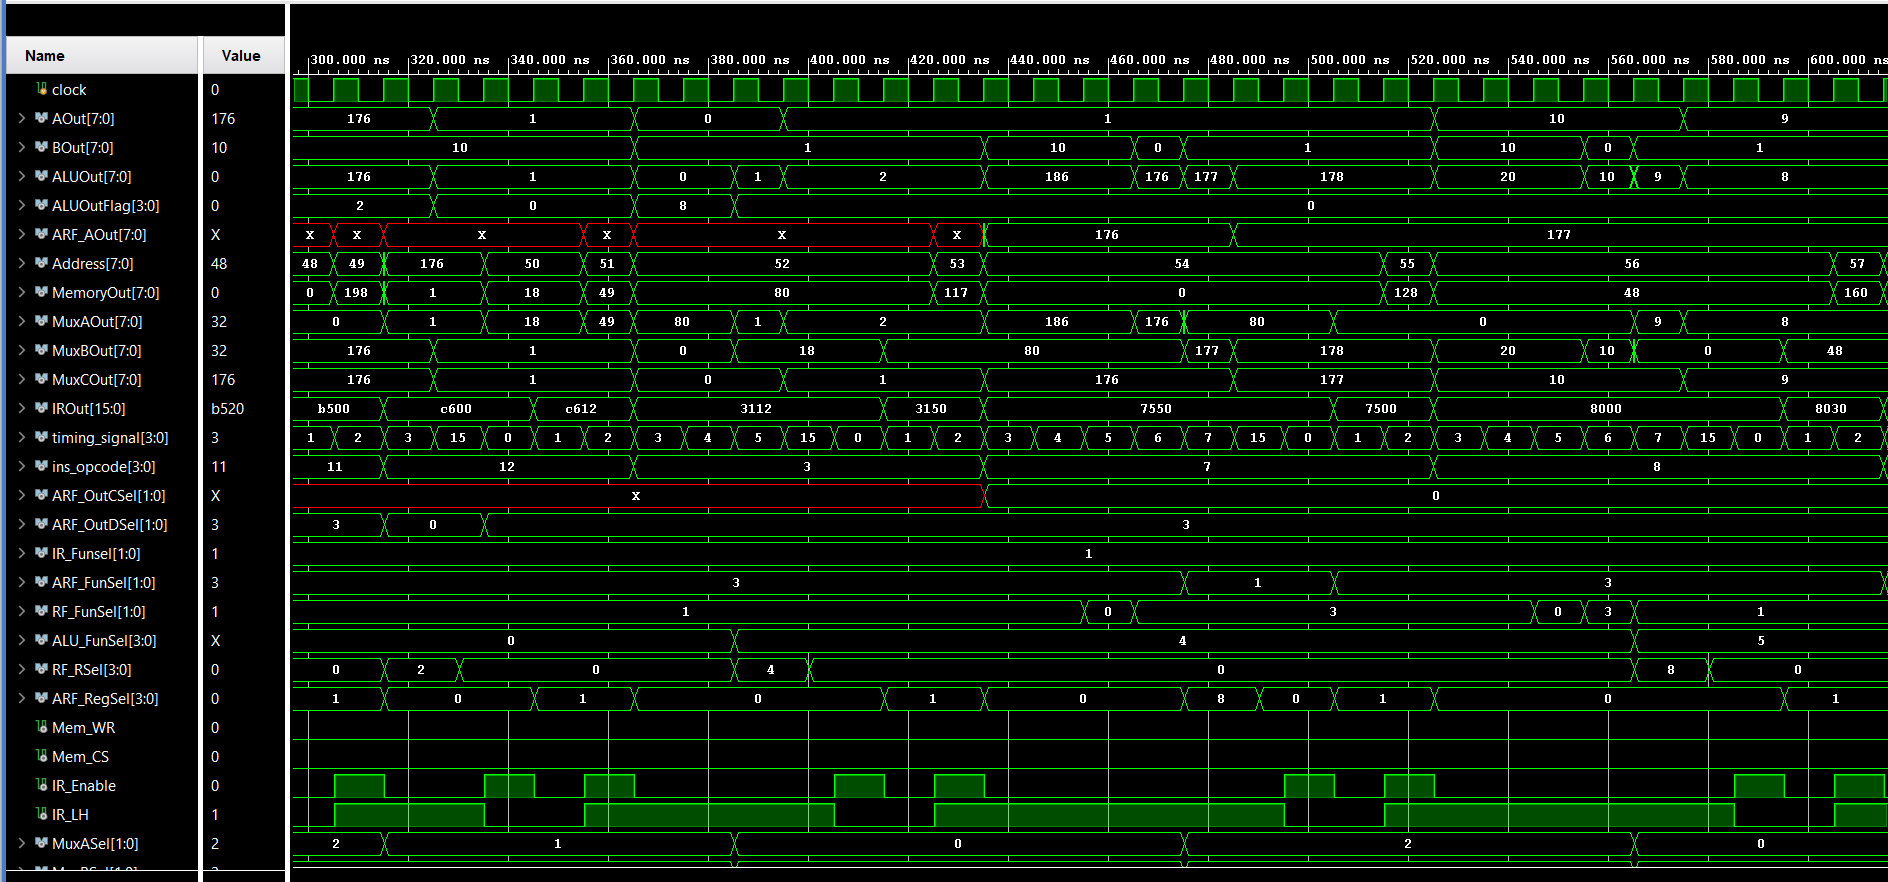
\includegraphics[width=1\textwidth]{photos/system_result_2.png}	
    \caption{simulation of system}
    \label{implementation}
\end{figure}


\begin{figure}[H]
    \centering
    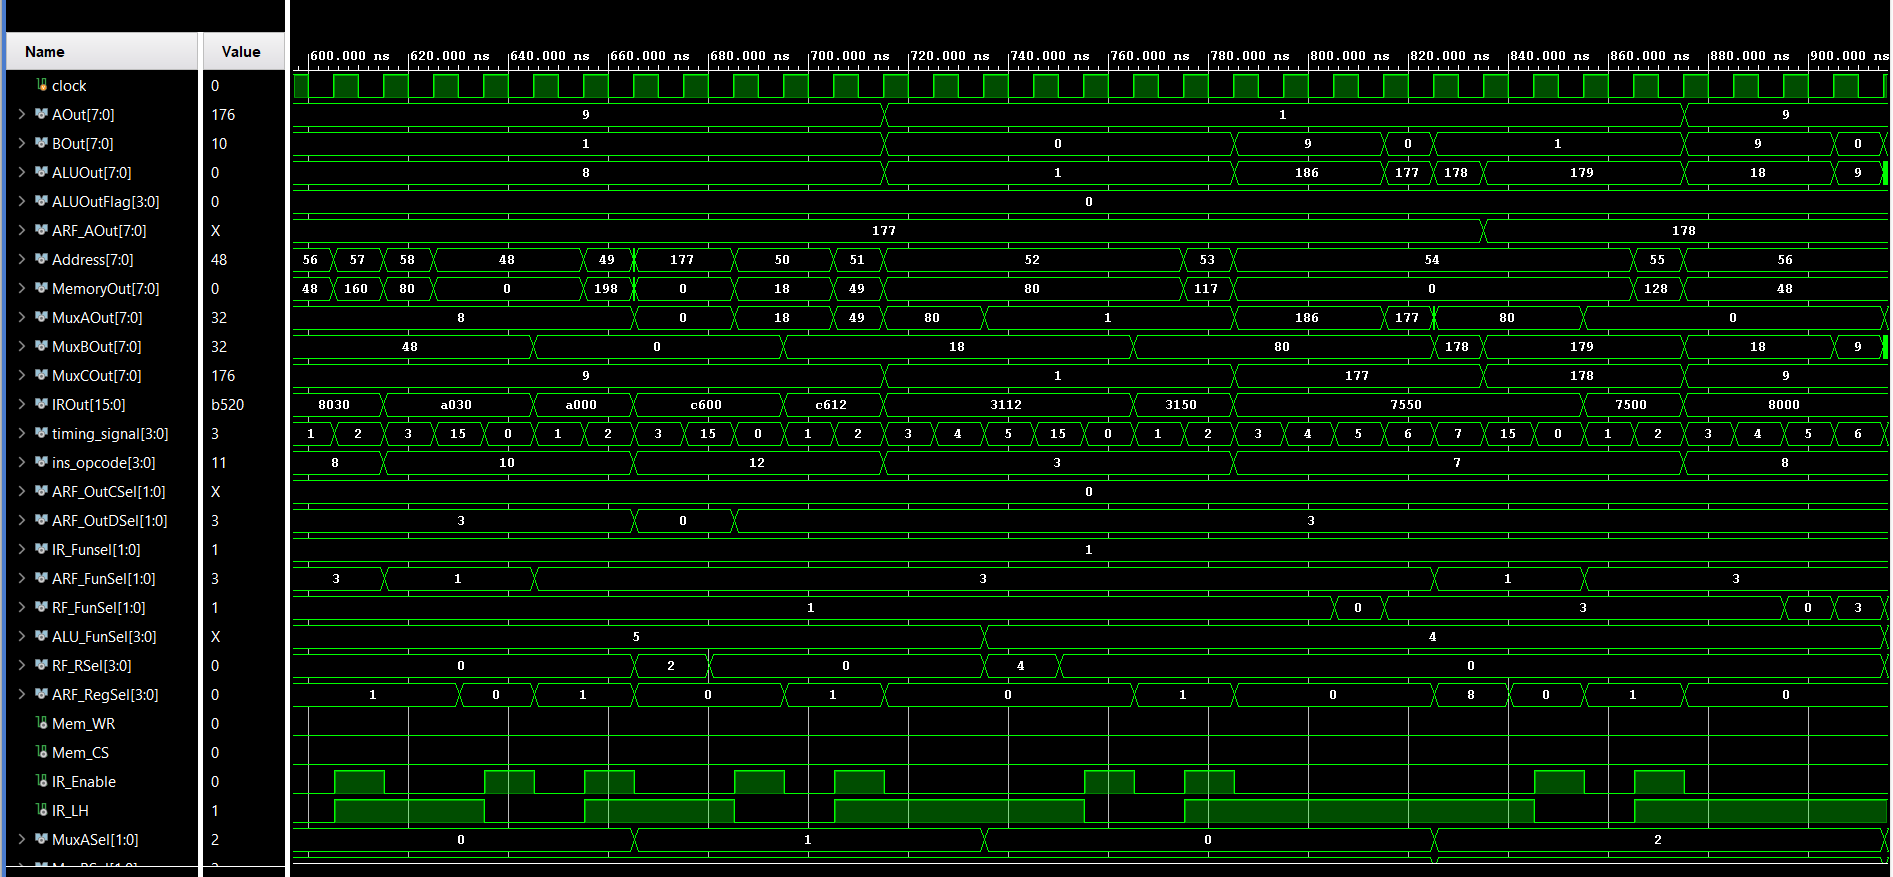
\includegraphics[width=1\textwidth]{photos/system_result_3.png}	
    \caption{simulation of system}
    \label{implementation}
\end{figure}



\begin{figure}[H]
    \centering
    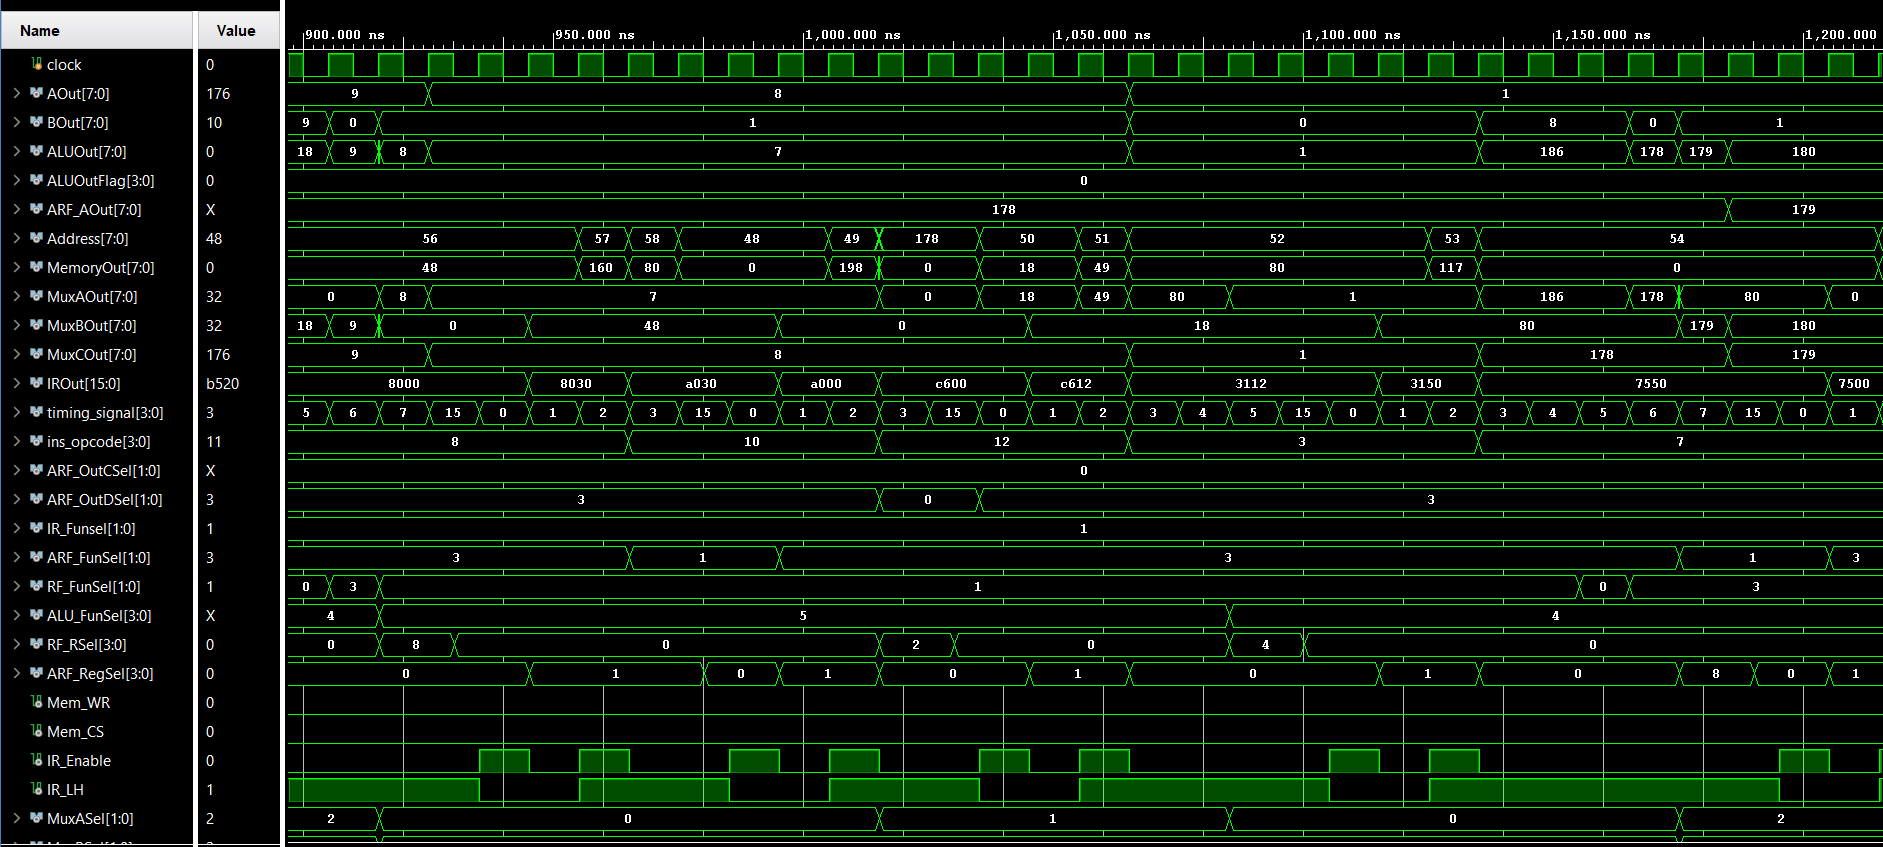
\includegraphics[width=1\textwidth]{photos/system_result_4.png}	
    \caption{simulation of system}
    \label{implementation}
\end{figure}

\begin{figure}[H]
    \centering
    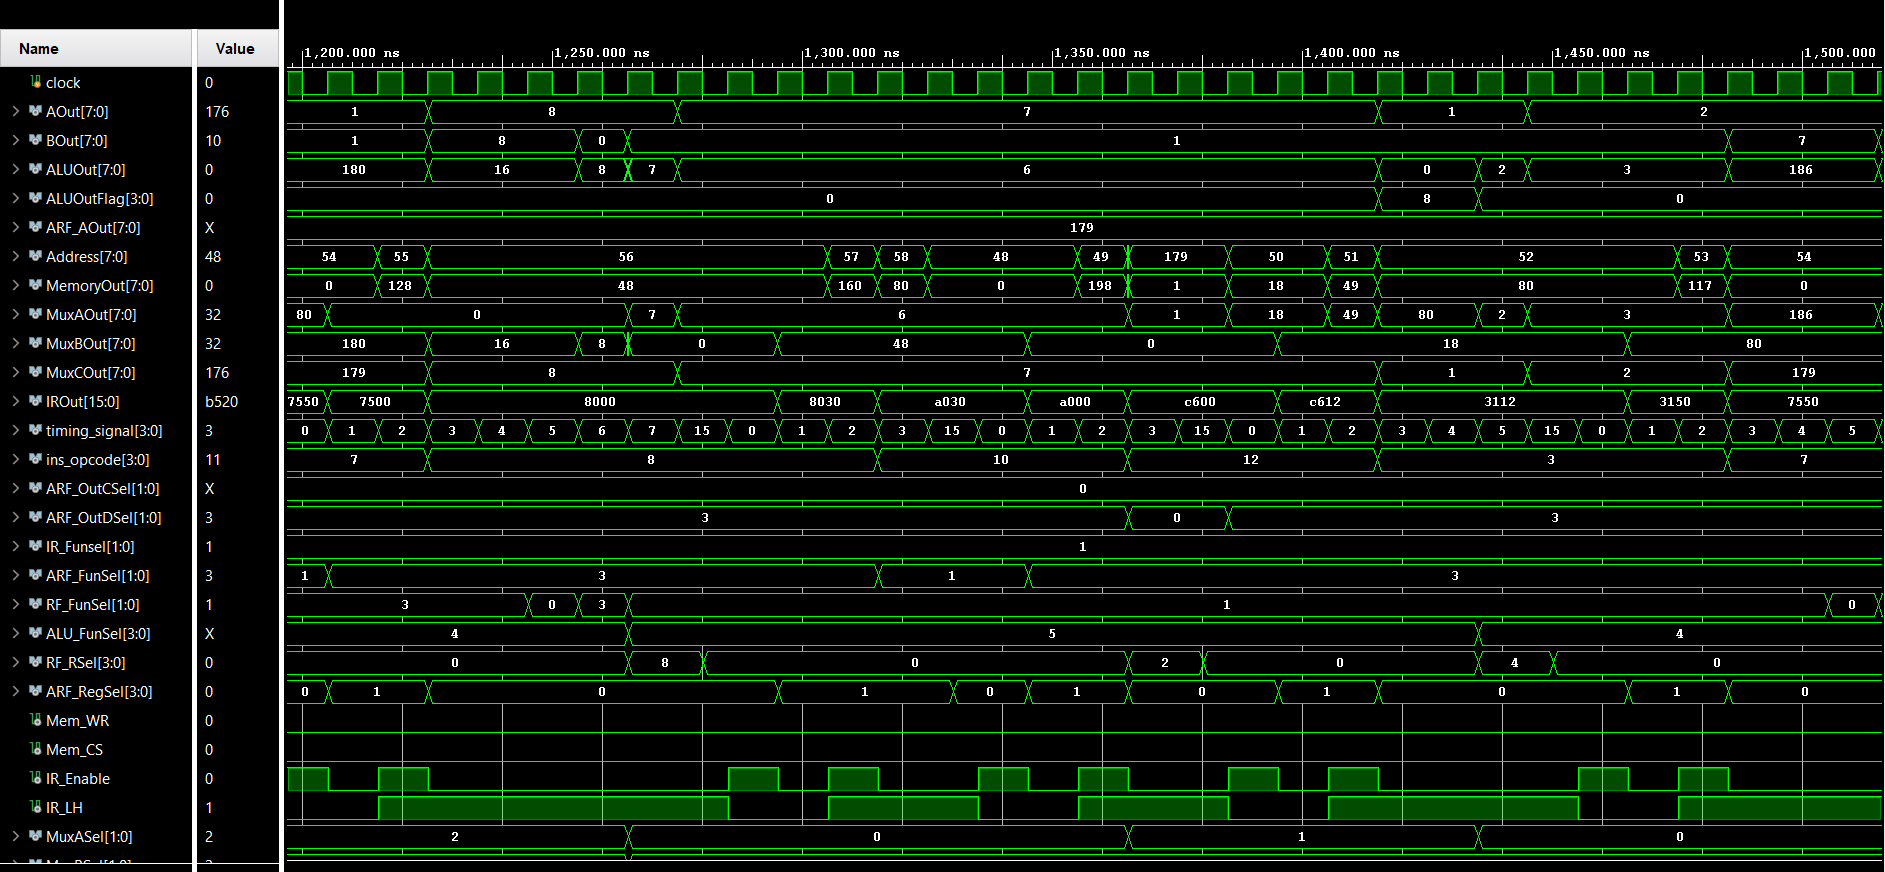
\includegraphics[width=1\textwidth]{photos/system_result_5.png}	
    \caption{simulation of system}
    \label{implementation}
\end{figure}


\begin{figure}[H]
    \centering
    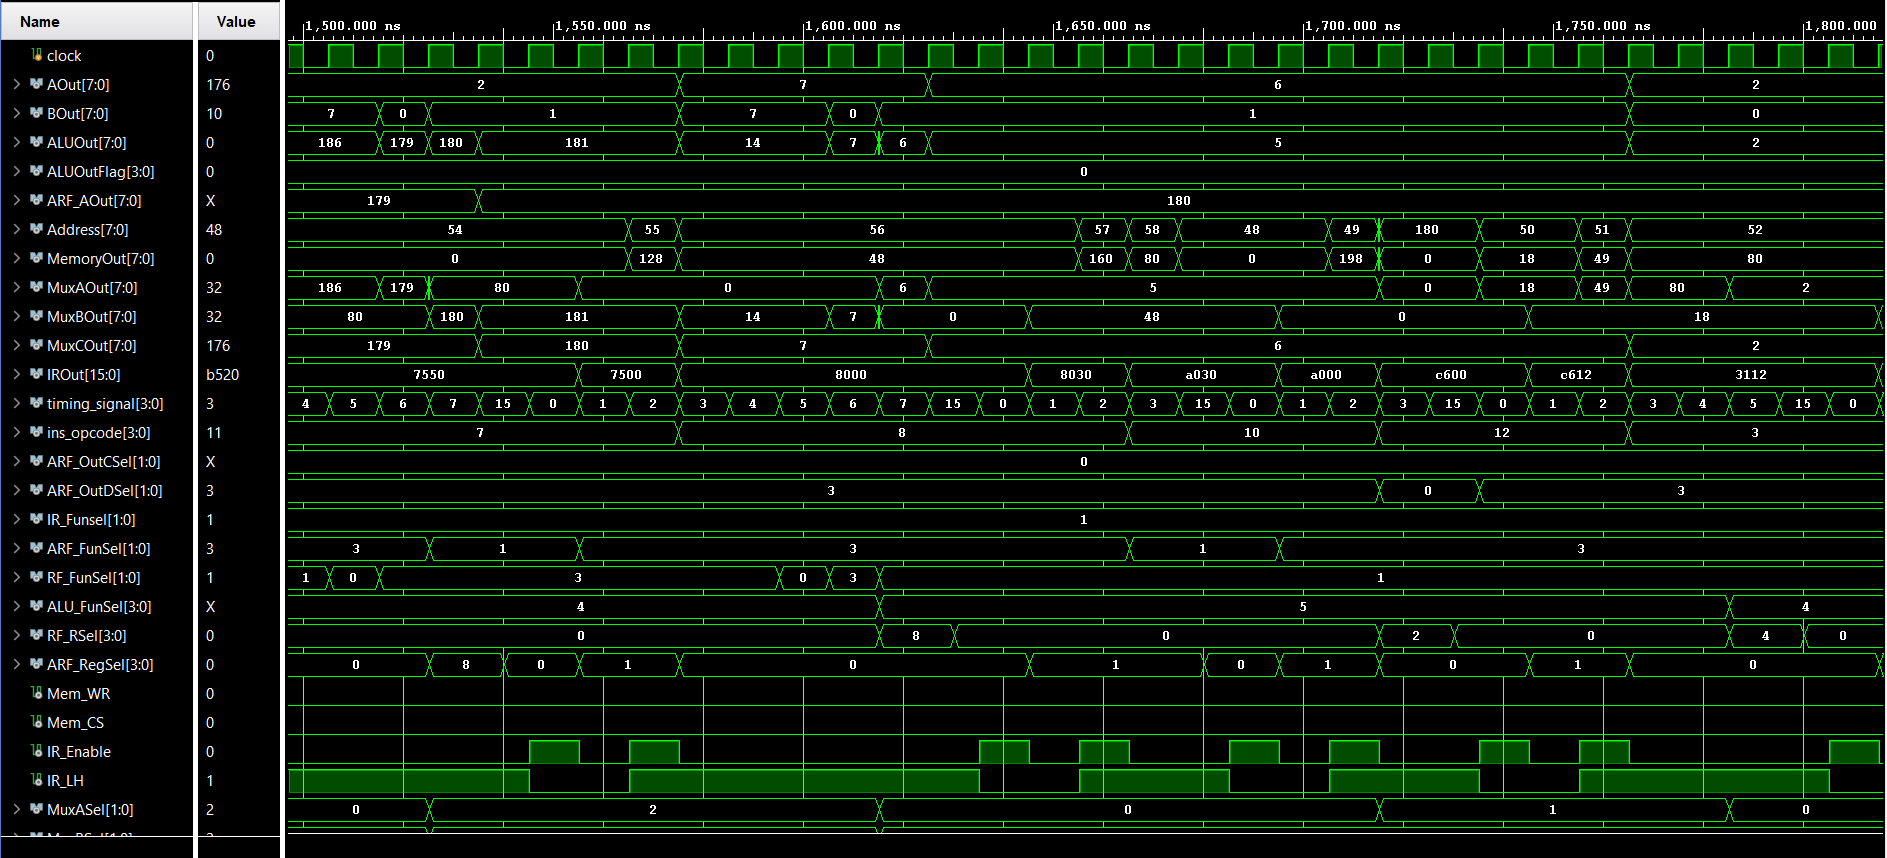
\includegraphics[width=1\textwidth]{photos/system_result_6.png}	
    \caption{simulation of system}
    \label{implementation}
\end{figure}


\begin{figure}[H]
    \centering
    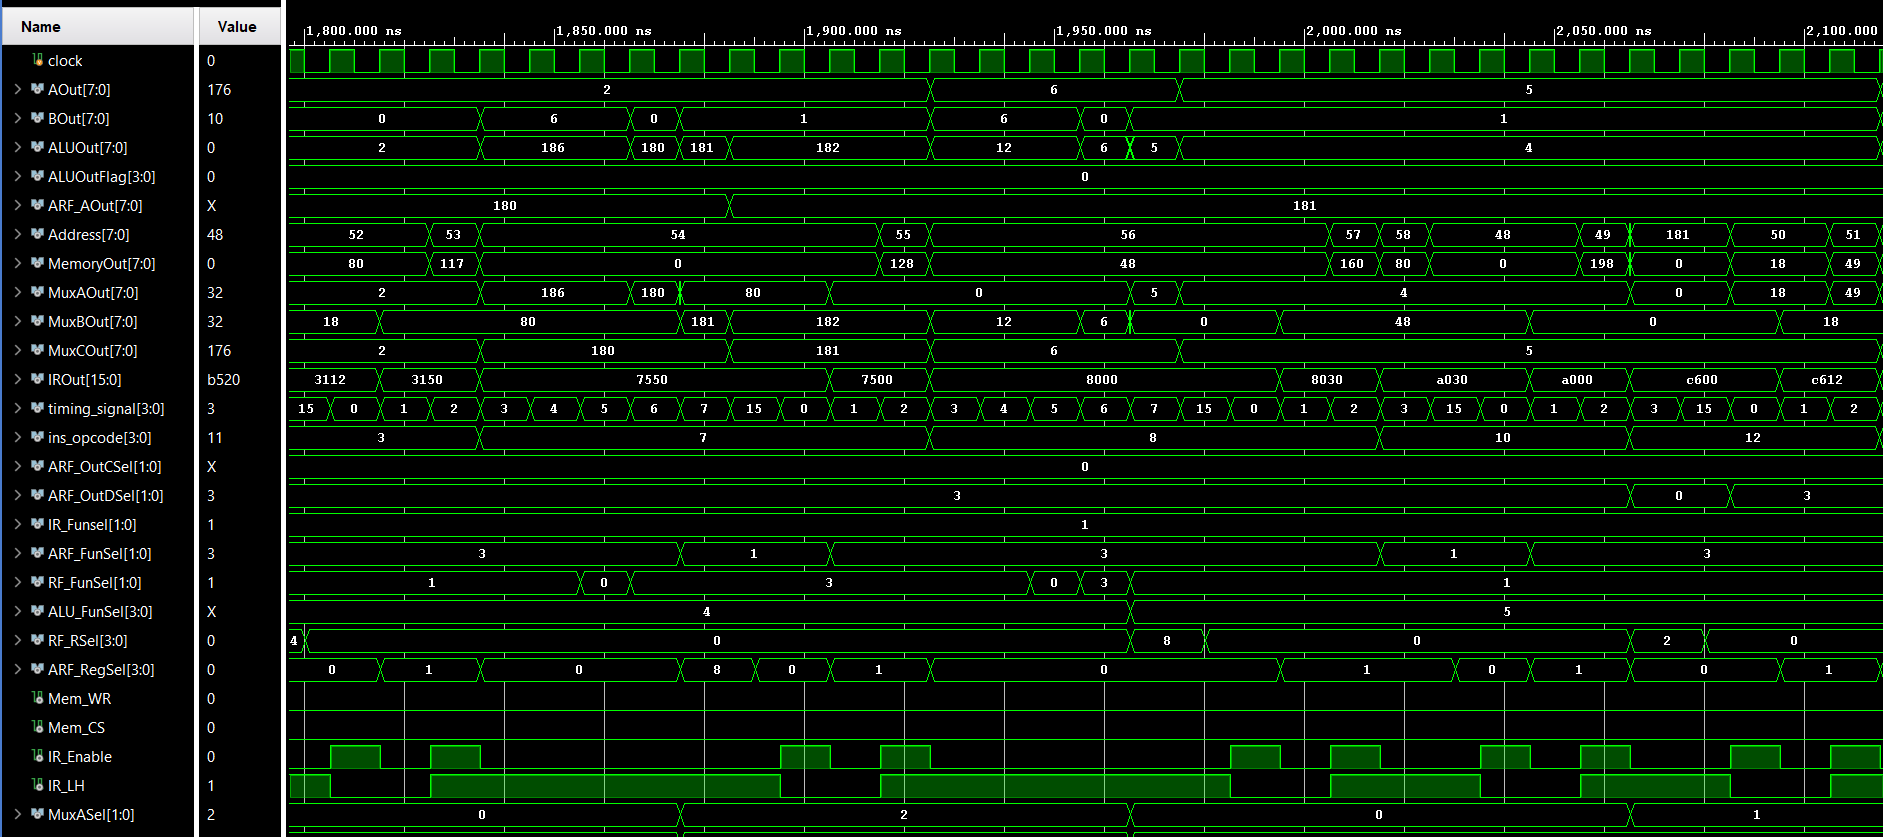
\includegraphics[width=1\textwidth]{photos/system_result_7.png}	
    \caption{simulation of system}
    \label{implementation}
\end{figure}

\begin{figure}[H]
    \centering
    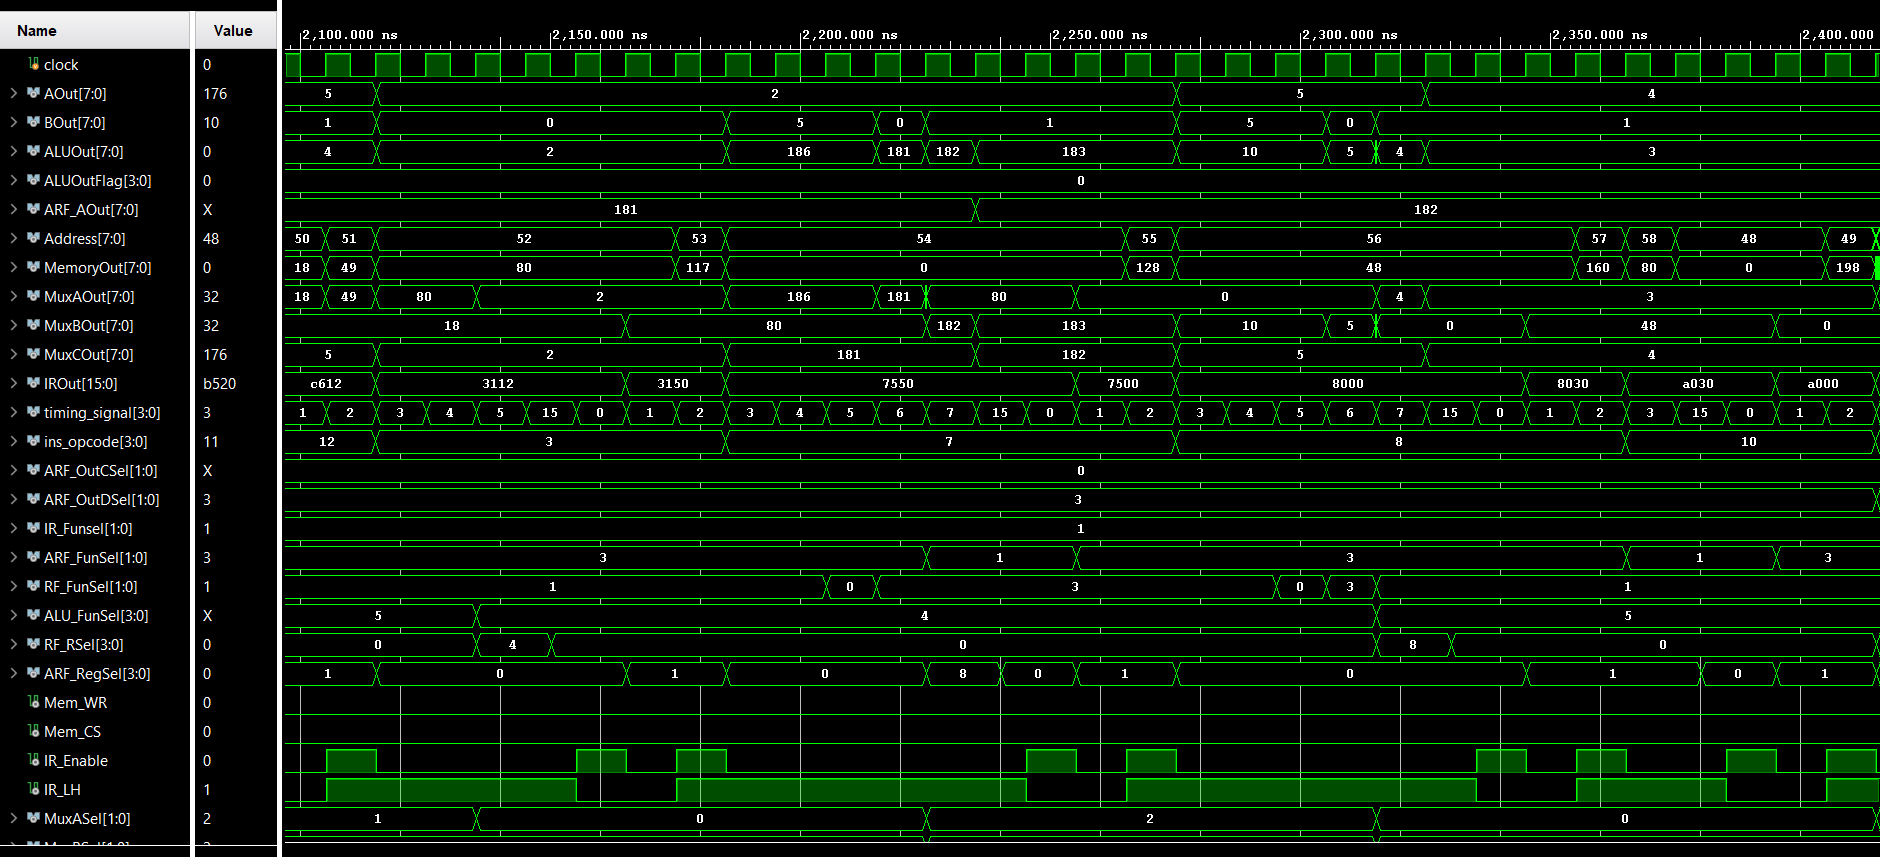
\includegraphics[width=1\textwidth]{photos/system_result_8.png}	
    \caption{simulation of system}
    \label{implementation}
\end{figure}

\begin{figure}[H]
    \centering
    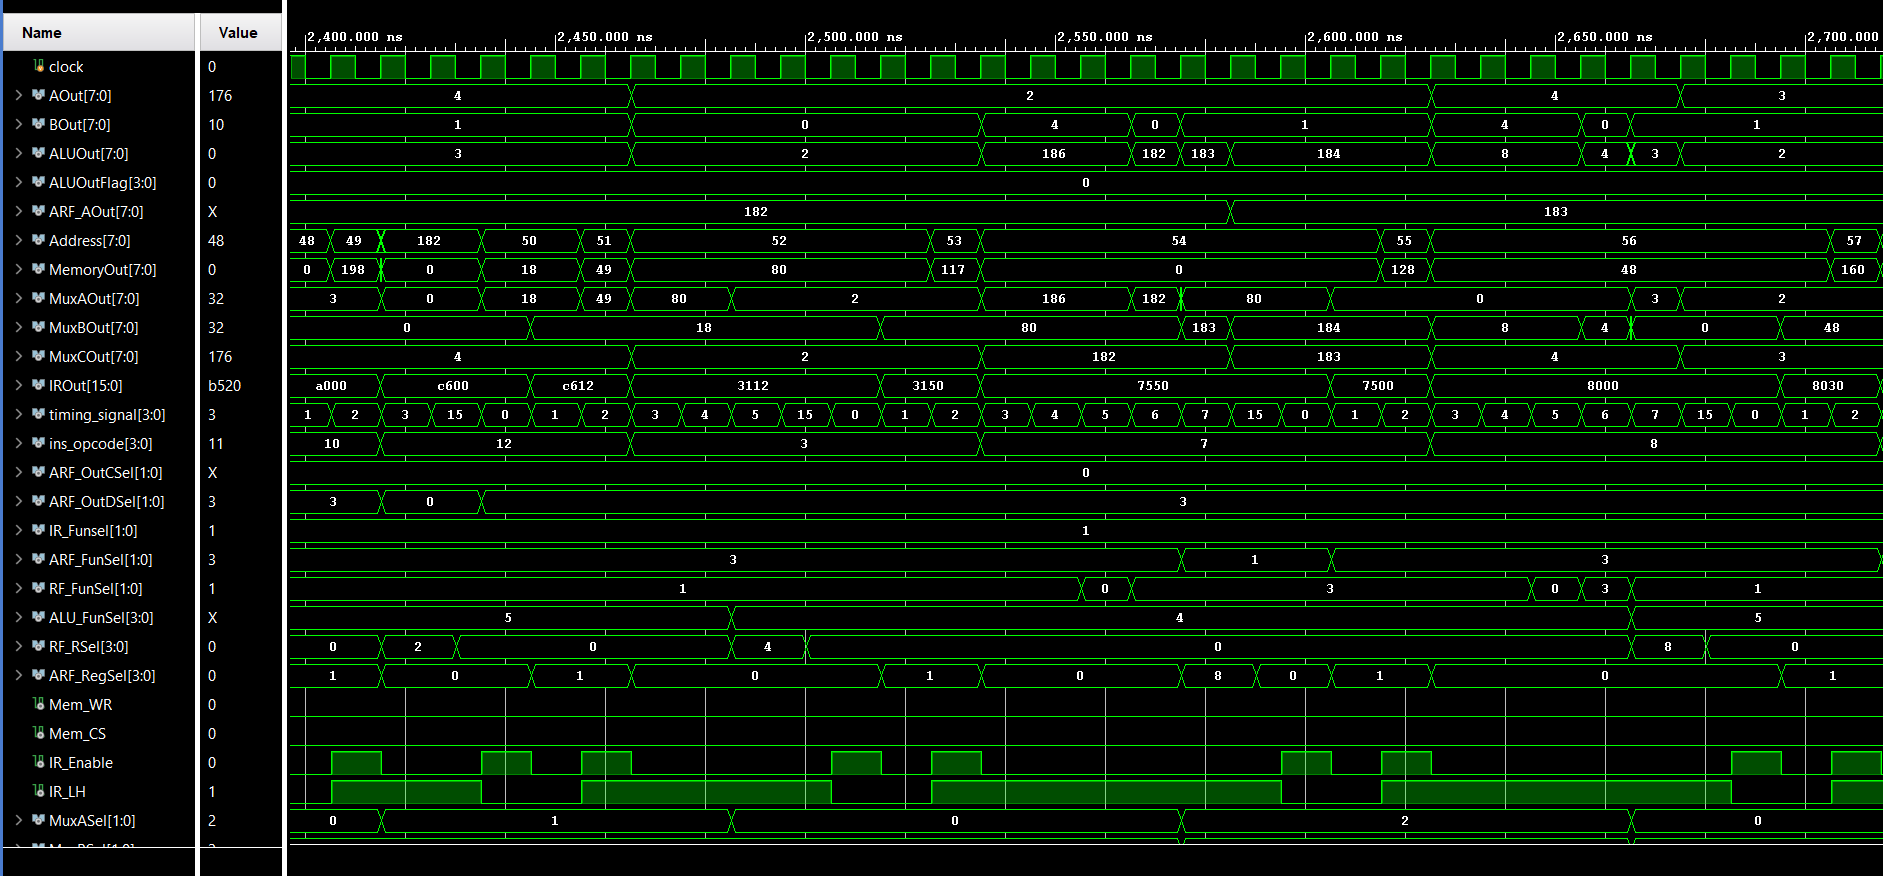
\includegraphics[width=1\textwidth]{photos/system_result_9.png}	
    \caption{simulation of system}
    \label{implementation}
\end{figure}

\begin{figure}[H]
    \centering
    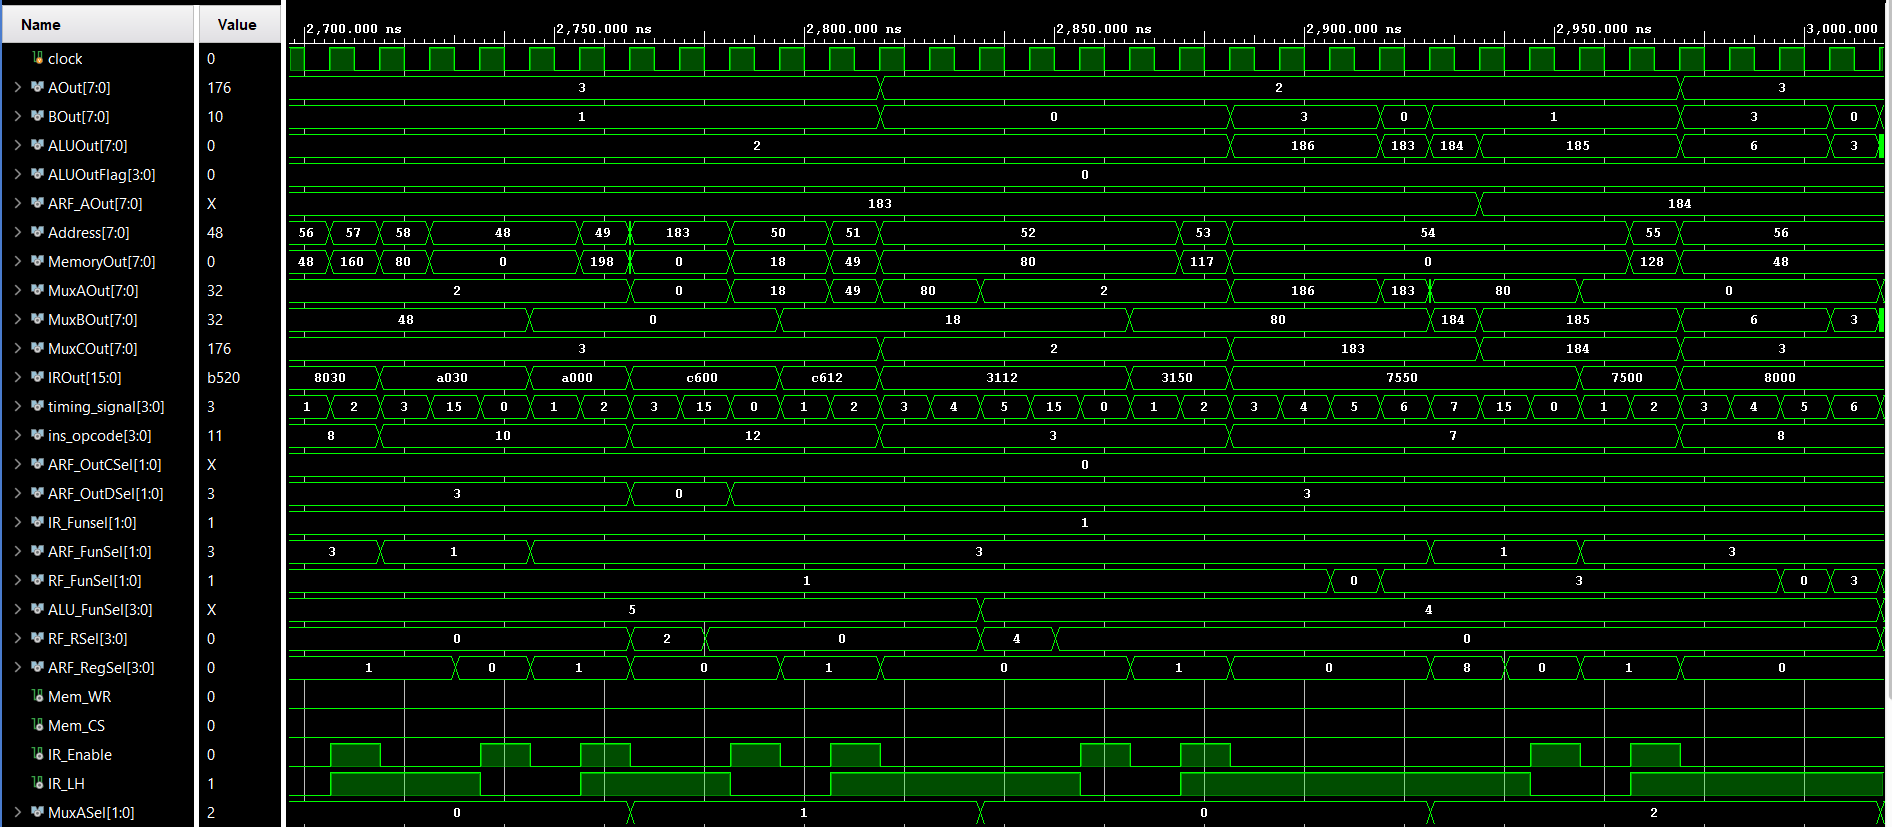
\includegraphics[width=1\textwidth]{photos/system_result_10.png}	
    \caption{simulation of system}
    \label{implementation}
\end{figure}

\begin{figure}[H]
    \centering
    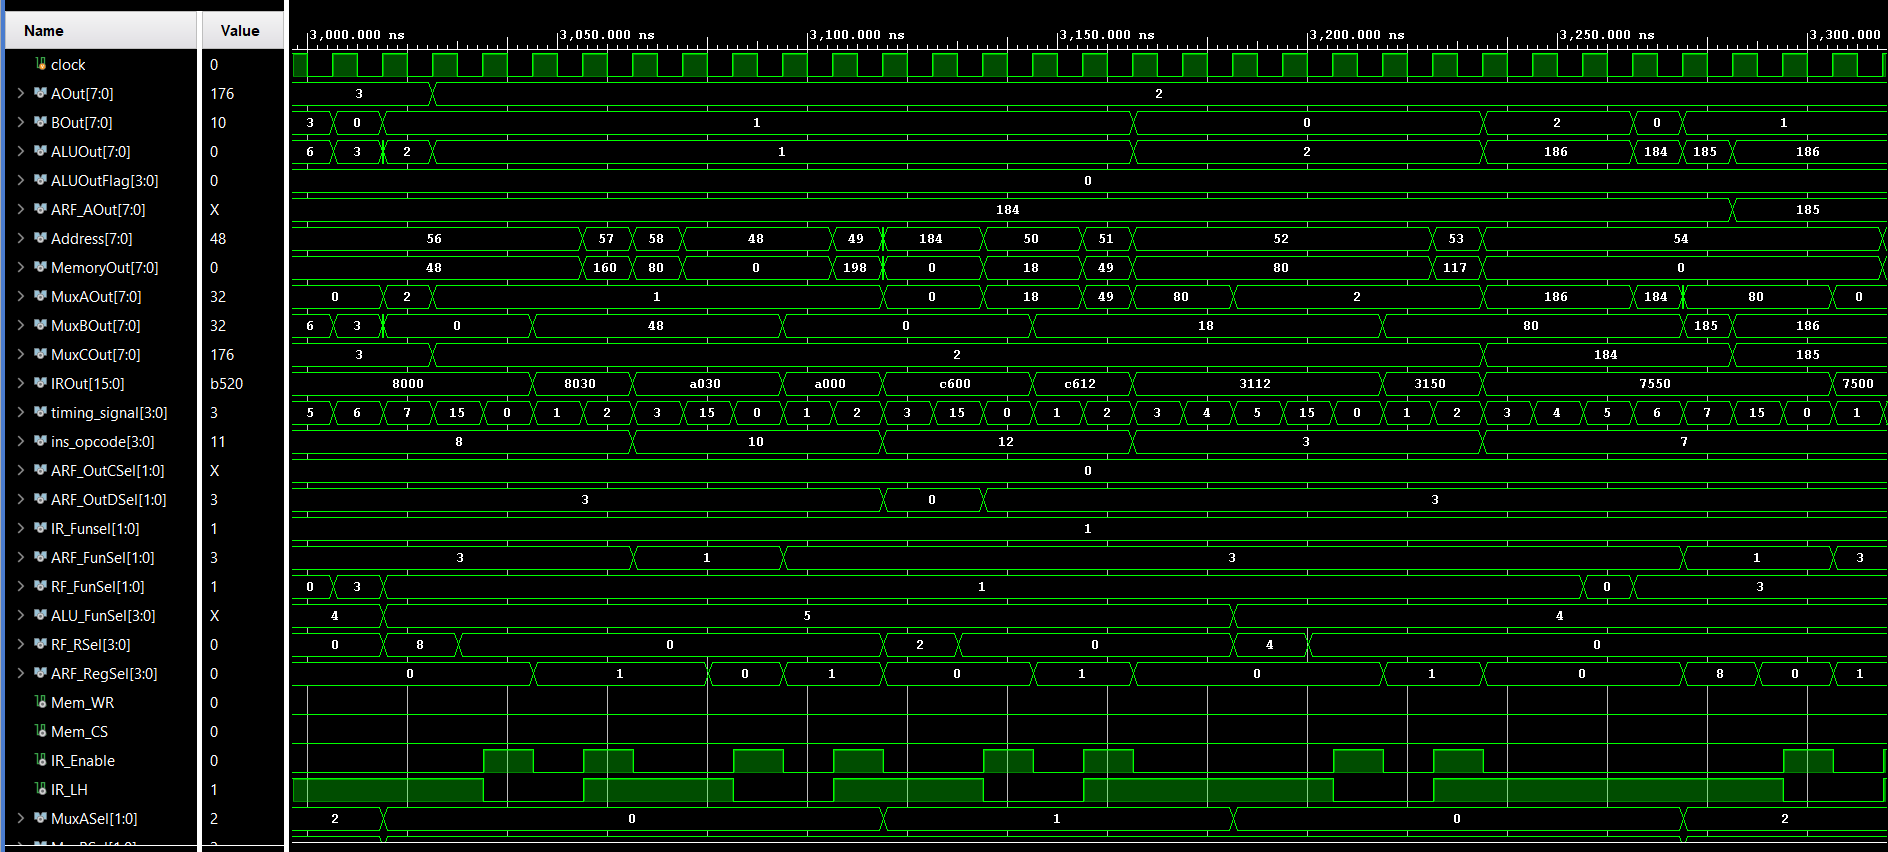
\includegraphics[width=1\textwidth]{photos/system_result_11.png}	
    \caption{simulation of system}
    \label{implementation}
\end{figure}

\begin{figure}[H]
    \centering
    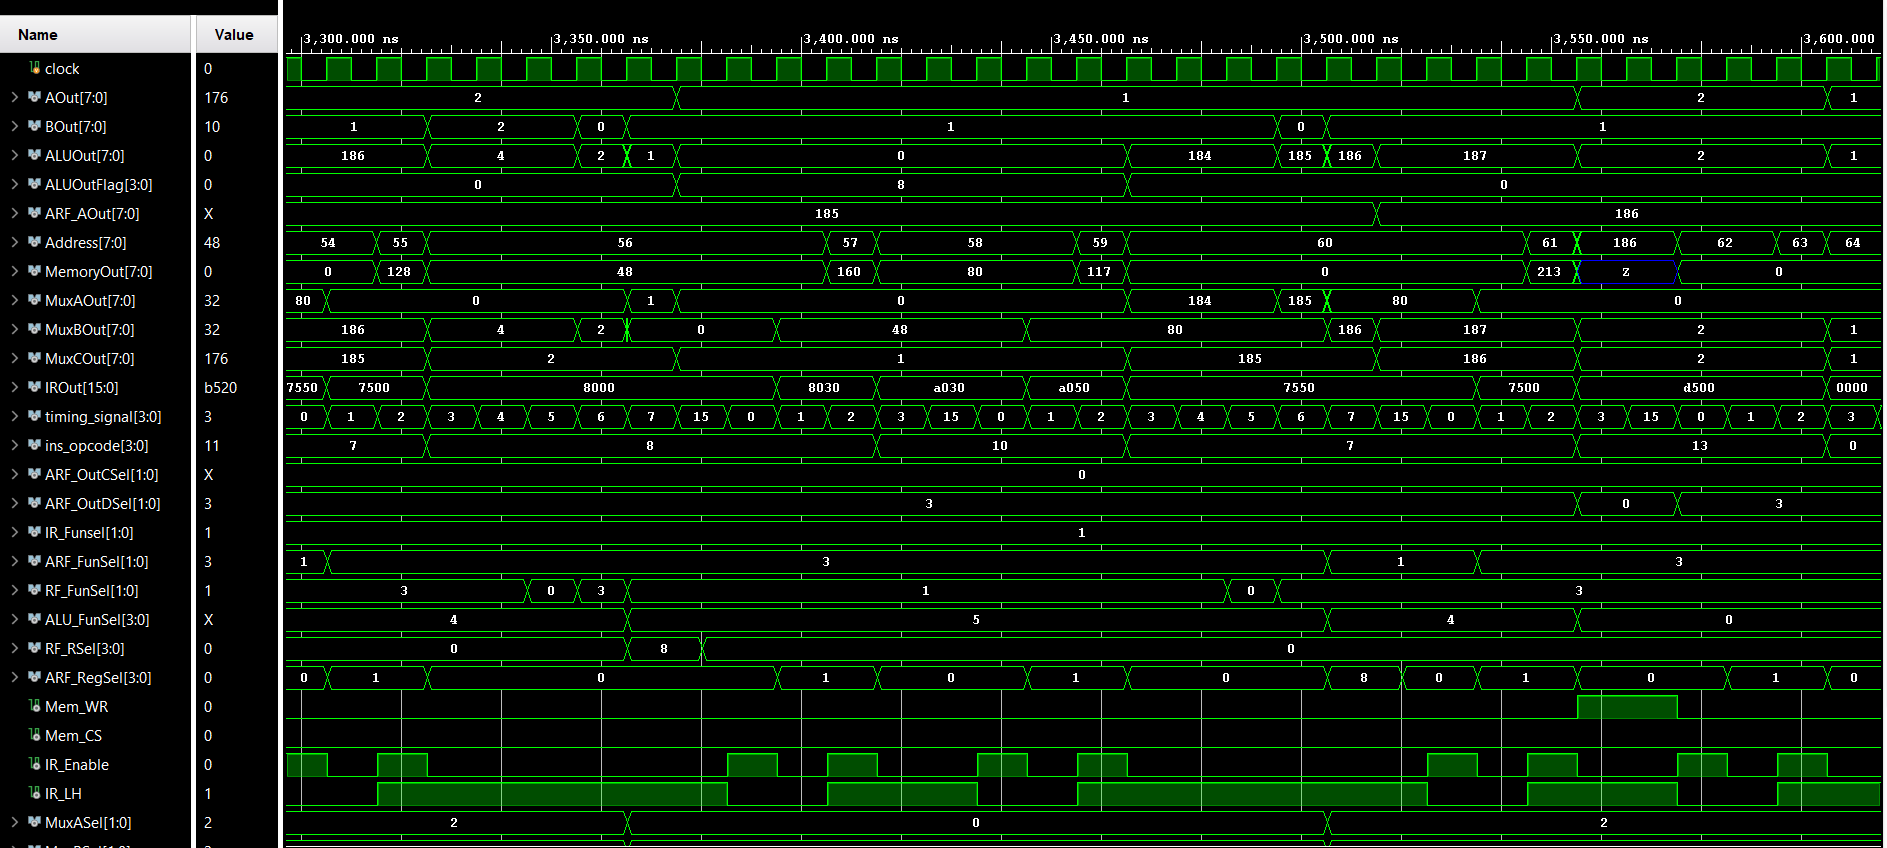
\includegraphics[width=1\textwidth]{photos/system_result_12.png}	
    \caption{simulation of system}
    \label{implementation}
\end{figure}

\begin{figure}[H]
    \centering
    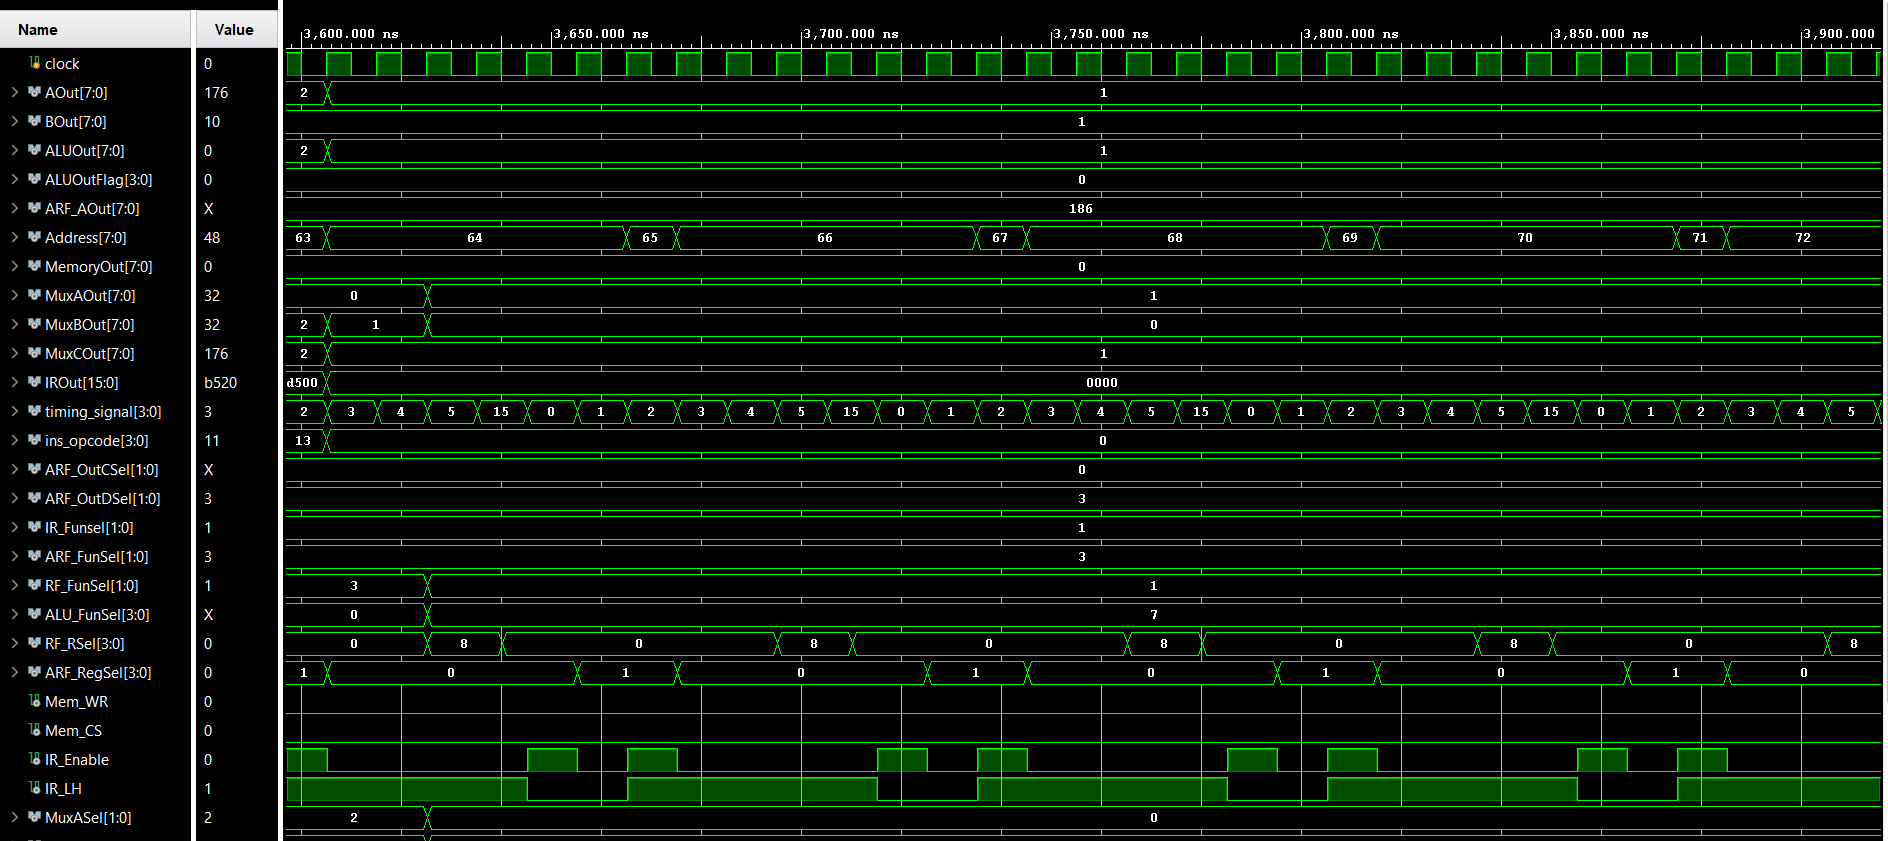
\includegraphics[width=1\textwidth]{photos/system_result_13.png}	
    \caption{simulation of system}
    \label{implementation}
\end{figure}



\section{DISCUSSION}
    In this project, we have implemented an ALU system which can take instructions defined in
Instruction Format. In order to achieve that, we have implemented a counter and by using counter's 
timing signal output, we have implemented fetch-decode operations and instructions' actual operations on
registers in register file and address register file. 

    We think we greatly achieve what we wanted. We successfully implemented fetch-decode operations
and instructions' actual operations defined in their OPCODE part. We've loaded our memory to instruction
register and used it in ALUSystem's components. While our code has worked, we couldn't run the last ST
operation successfully. While we achieve the adding numbers in memory from 0xB0 to 0xBA, we couldn't store it
in memory. It is because we couldn't find a way to write value into the memory. But our success can be seen
from the simulation bar.

    While doing this homework, we have encountered with a lot of difficulties. One of them is our one teamfriend, Emre,
were in another city, it maked our job difficult, but we've overcomed it by giving less tasks to our teamfriend
that is in another city.

    Another big difficult was debugging. Finding the root of problems has caused us to lose a lot of days.
We've encountered with a lot of different problems. Syncing the clock with code was the hardest task.
Another big problem was ensuring the security. Without security, we have overwrite some registers and
didn't realize it. Enhancing security has provideded our code to be safe. 

    The other issue was the limited time. 5 ns clock was not enough for us to simulate all the loop. In order to
overcome it, we have adjusted the simulation time in setting by changing xsim.simulation.runtime to 4000 ns. Default is
1000 ns.

    We have learned how an instructor is performed in the computer, and its relates with clock cycles and ALU components.



\section{CONCLUSION}
In this project we designed a hardwired control unit with the help of the system module we created in the
first project. We designed a simple fetch-decode-execute cycle which is capable of doing non addressing
mode instructions such as arithmetic and logic operations on registers, as well as operations having an
addressing mode such as loading a value from the memory or storing a value into the memory.

During this project, we communicated using whatsapp and we used GitHub to help each other fix some 
mistakes we made. Some operations took more than one cycle to complete, therefore we needed to arrange 
the timing accordingly. We needed to re-design the fetch cycle and conditions to increment the counters 
to make the system work properly. The error checking was challenging for this project as we needed to 
check each step over and over again to find what might be the cause of an error. 

\end{document}